\begin{figure}[ht]
    \centering
    \begin{tikzpicture}[node distance=1.5cm and 1cm, auto]
        % Nodo per immagine 1 con didascalia sotto
        \node (img1) {
            \begin{tabular}{c}
                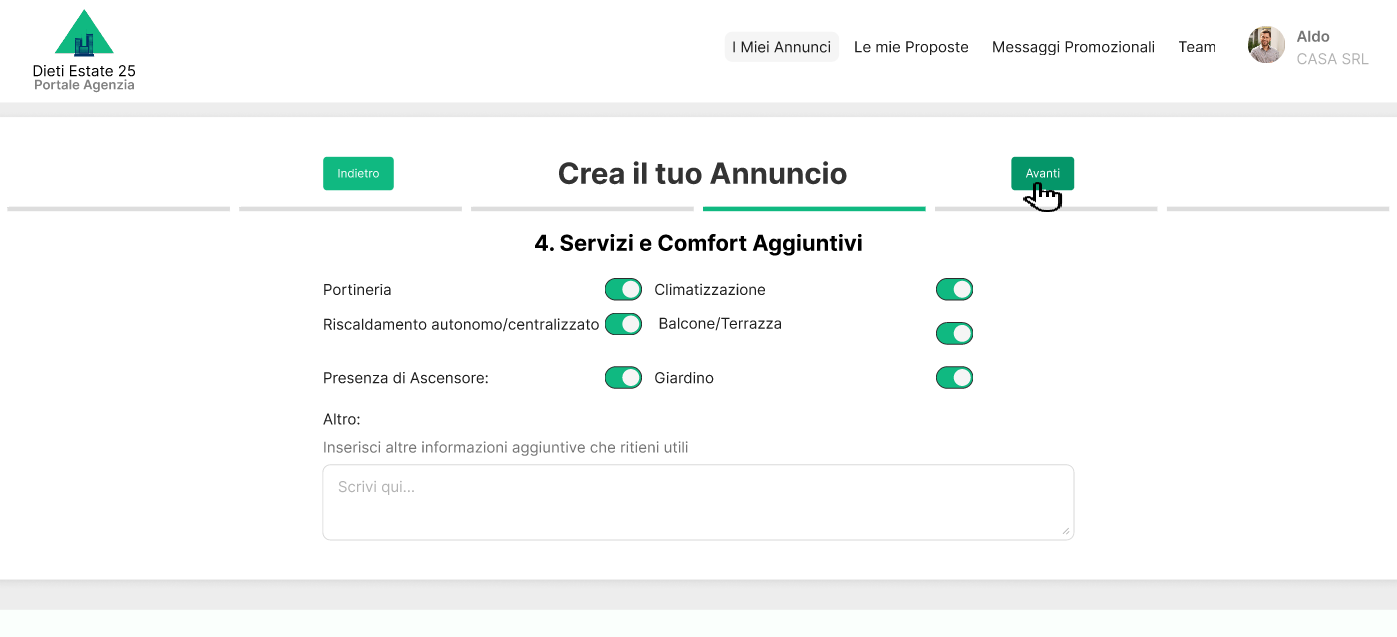
\includegraphics[width=\textwidth,keepaspectratio]{Immagini/Mockup/aggiungi annuncio/scenario principale/step4.png} \\
                Cockburn: step 4/5
            \end{tabular}
        };
        
        % Nodo per immagine 2 con didascalia sotto, posizionato a destra di img1
        \node (img2) [below=of img1] {
            \begin{tabular}{c}
                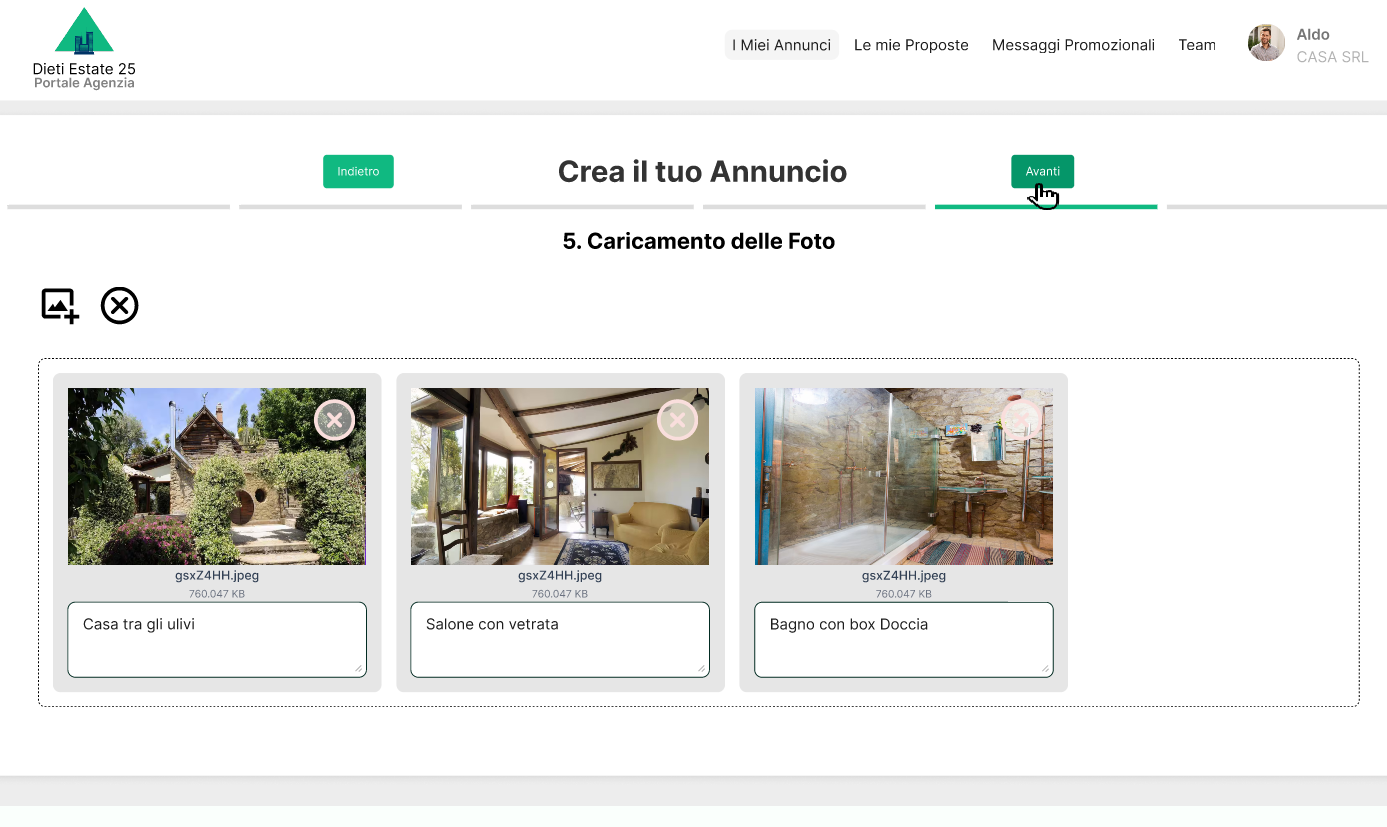
\includegraphics[width=\textwidth,keepaspectratio]{Immagini/Mockup/aggiungi annuncio/scenario principale/step5.png} \\
                Cockburn: step 6
            \end{tabular}
        };
        
        % Disegna le frecce
        \draw[->, thick] (img1) -- (img2);
      
    \end{tikzpicture}
    \caption{Mockup: scenario principale della tabella di Cockburn del caso d'uso nuovo annuncio.}
    \label{fig:mockup_scenario_principale_parte2_aggiungi_annuncio}
\end{figure}

\newpage

\input{Requisiti Del Software/Analisi dei Requisiti/Mockup/aggiungi annuncio/scenario principale Parte III}

